\question{Газовые лазеры. Эксимерные лазеры}
Генерация осуществляется на переходах со связывающих электронных термов 
(верхнее состояние) на разлётный электронный терм (нижнее состояние) так 
называемых эксимерных молекул, то есть молекул, существующих устойчиво только 
в возбуждённом состоянии. Примером эксимерных молекул являются димеры атомов 
благородных газов, их галогениды и т.п. Наличие эксимерных молекул 
эквивалентно инверсии, поэтому она достигается созданием эксимерных молекул. 
Оно происходит под действием пучка быстрых электронов или в газовом разряде. 
Опустошение нижнего уровня происходит автоматически, так как молекулы, 
попавшие в нижнее состояние, распадаются.

\begin{figure}[h]
    \center
    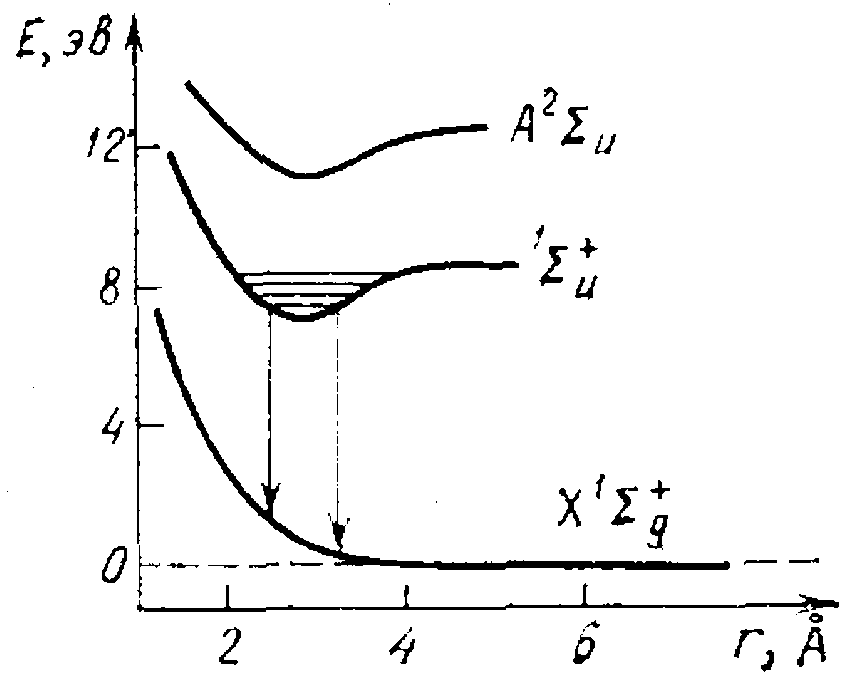
\includegraphics[width=.47\textwidth]{25}
    \caption{Уровни энергии эксимера \( Xe_2^* \)}
\end{figure}

Диапазон генерации эксимерных лазеров простирается от видимого света до 
вакуумного ультрафиолета. Наибольшее применение нашли 
\( XeF-,\ XeCl-,\ KrF-,\ KrCl- \)лазеры, работающие на длинах волн 352, 
308, 249 и 222 нм соответственно.

Характерной чертой этих лазеров является полная незаселённость нижнего уровня